% SOURCE: edit-harness/results/frame_a/cells/p2_llama-3.2-1b_real_MIX_C.json + provenance_v2_report.json
% !TEX encoding = UTF-8 Unicode
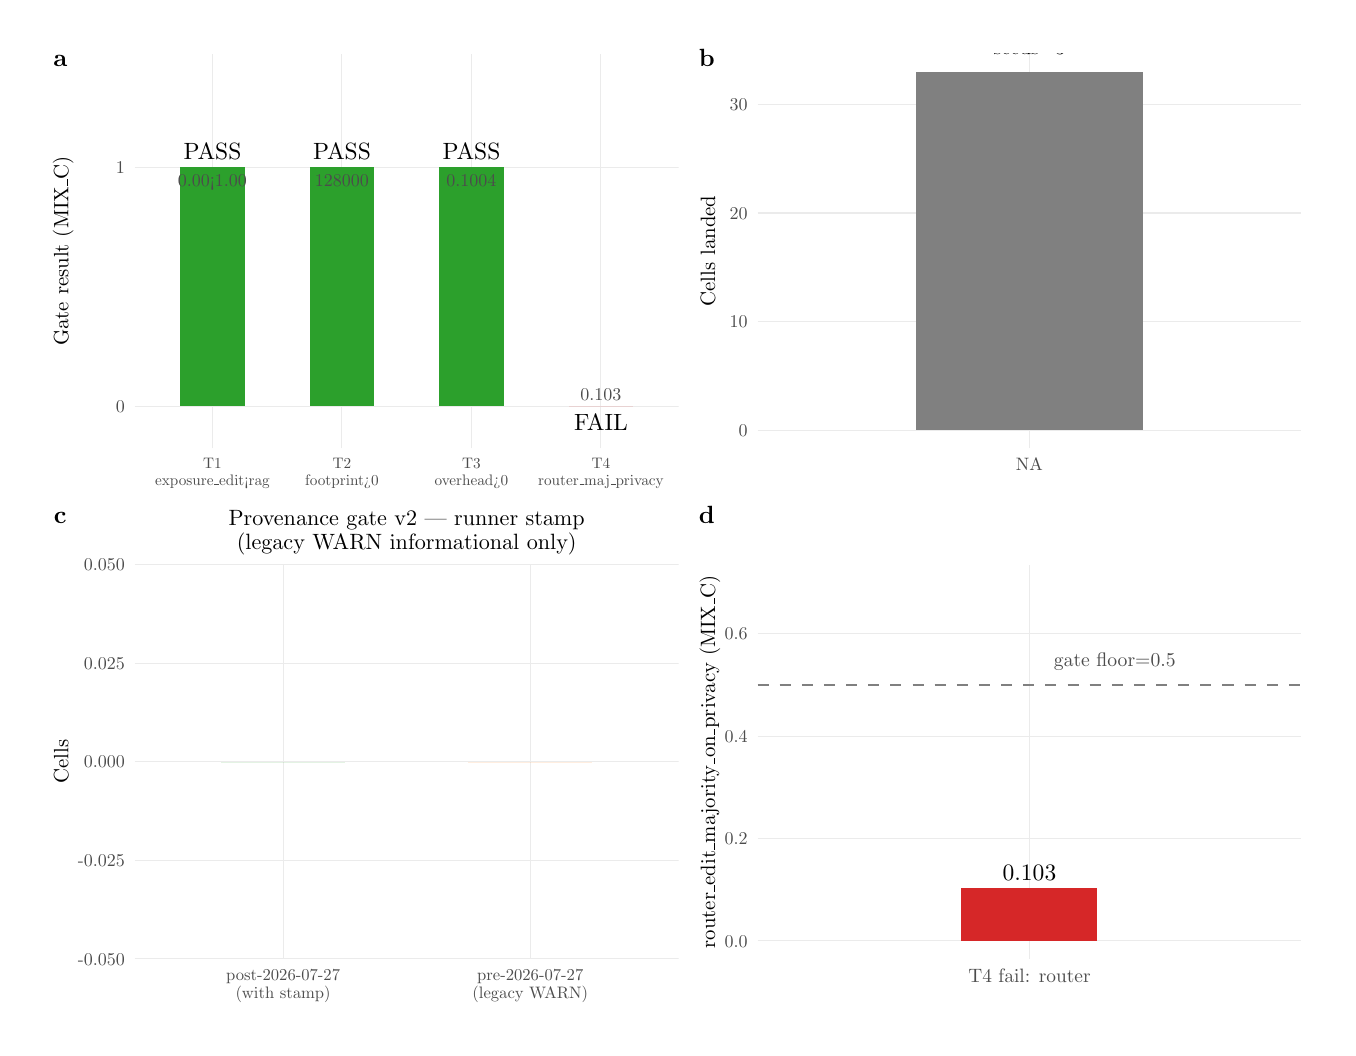
\begin{tikzpicture}[x=1pt,y=1pt]
\definecolor{fillColor}{RGB}{255,255,255}
\path[use as bounding box,fill=fillColor,fill opacity=0.00] (0,0) rectangle (469.75,361.35);
\begin{scope}
\path[clip] (  0.00,  0.00) rectangle (469.75,361.35);
\definecolor{drawColor}{RGB}{255,255,255}
\definecolor{fillColor}{RGB}{255,255,255}

\path[draw=drawColor,line width= 0.6pt,line join=round,line cap=round,fill=fillColor] (  0.00,  0.00) rectangle (469.76,361.35);
\end{scope}
\begin{scope}
\path[clip] (  5.50,191.02) rectangle (239.21,355.85);
\definecolor{fillColor}{RGB}{255,255,255}

\path[fill=fillColor] (  5.50,191.02) rectangle (239.21,355.85);
\end{scope}
\begin{scope}
\path[clip] (239.21,191.02) rectangle (464.25,355.85);
\definecolor{fillColor}{RGB}{255,255,255}

\path[fill=fillColor] (239.21,191.02) rectangle (464.25,355.85);
\end{scope}
\begin{scope}
\path[clip] (  5.50,  5.50) rectangle (239.21,191.02);
\definecolor{fillColor}{RGB}{255,255,255}

\path[fill=fillColor] (  5.50,  5.50) rectangle (239.21,191.02);
\end{scope}
\begin{scope}
\path[clip] (239.21,  5.50) rectangle (464.25,191.02);
\definecolor{fillColor}{RGB}{255,255,255}

\path[fill=fillColor] (239.21,  5.50) rectangle (464.25,191.02);
\end{scope}
\begin{scope}
\path[clip] ( 38.69,209.42) rectangle (235.21,351.85);
\definecolor{drawColor}{gray}{0.92}

\path[draw=drawColor,line width= 0.4pt,line join=round] ( 38.69,224.52) --
	(235.21,224.52);

\path[draw=drawColor,line width= 0.4pt,line join=round] ( 38.69,310.85) --
	(235.21,310.85);

\path[draw=drawColor,line width= 0.4pt,line join=round] ( 66.77,209.42) --
	( 66.77,351.85);

\path[draw=drawColor,line width= 0.4pt,line join=round] (113.56,209.42) --
	(113.56,351.85);

\path[draw=drawColor,line width= 0.4pt,line join=round] (160.35,209.42) --
	(160.35,351.85);

\path[draw=drawColor,line width= 0.4pt,line join=round] (207.14,209.42) --
	(207.14,351.85);
\definecolor{fillColor}{RGB}{44,160,44}

\path[fill=fillColor] ( 55.07,224.52) rectangle ( 78.46,310.85);

\path[fill=fillColor] (101.86,224.52) rectangle (125.25,310.85);

\path[fill=fillColor] (148.65,224.52) rectangle (172.04,310.85);
\definecolor{fillColor}{RGB}{214,39,40}

\path[fill=fillColor] (195.44,224.52) rectangle (218.83,224.52);
\definecolor{drawColor}{RGB}{0,0,0}

\node[text=drawColor,anchor=base,inner sep=0pt, outer sep=0pt, scale=  0.85] at ( 66.77,313.79) {PASS};

\node[text=drawColor,anchor=base,inner sep=0pt, outer sep=0pt, scale=  0.85] at (113.56,313.79) {PASS};

\node[text=drawColor,anchor=base,inner sep=0pt, outer sep=0pt, scale=  0.85] at (160.35,313.79) {PASS};

\node[text=drawColor,anchor=base,inner sep=0pt, outer sep=0pt, scale=  0.85] at (207.14,215.70) {FAIL};
\definecolor{drawColor}{gray}{0.30}

\node[text=drawColor,anchor=base,inner sep=0pt, outer sep=0pt, scale=  0.65] at ( 66.77,304.09) {0.00<1.00};

\node[text=drawColor,anchor=base,inner sep=0pt, outer sep=0pt, scale=  0.65] at (113.56,304.09) {128000};

\node[text=drawColor,anchor=base,inner sep=0pt, outer sep=0pt, scale=  0.65] at (160.35,304.09) {0.1004};

\node[text=drawColor,anchor=base,inner sep=0pt, outer sep=0pt, scale=  0.65] at (207.14,226.78) {0.103};
\end{scope}
\begin{scope}
\path[clip] (  0.00,  0.00) rectangle (469.75,361.35);
\definecolor{drawColor}{gray}{0.30}

\node[text=drawColor,anchor=base east,inner sep=0pt, outer sep=0pt, scale=  0.65] at ( 35.09,222.28) {0};

\node[text=drawColor,anchor=base east,inner sep=0pt, outer sep=0pt, scale=  0.65] at ( 35.09,308.61) {1};
\end{scope}
\begin{scope}
\path[clip] (  0.00,  0.00) rectangle (469.75,361.35);
\definecolor{drawColor}{gray}{0.30}

\node[text=drawColor,anchor=base,inner sep=0pt, outer sep=0pt, scale=  0.55] at ( 66.77,202.03) {T1};

\node[text=drawColor,anchor=base,inner sep=0pt, outer sep=0pt, scale=  0.55] at ( 66.77,196.09) {exposure\_edit<rag};

\node[text=drawColor,anchor=base,inner sep=0pt, outer sep=0pt, scale=  0.55] at (113.56,202.03) {T2};

\node[text=drawColor,anchor=base,inner sep=0pt, outer sep=0pt, scale=  0.55] at (113.56,196.09) {footprint>0};

\node[text=drawColor,anchor=base,inner sep=0pt, outer sep=0pt, scale=  0.55] at (160.35,202.03) {T3};

\node[text=drawColor,anchor=base,inner sep=0pt, outer sep=0pt, scale=  0.55] at (160.35,196.09) {overhead>0};

\node[text=drawColor,anchor=base,inner sep=0pt, outer sep=0pt, scale=  0.55] at (207.14,202.03) {T4};

\node[text=drawColor,anchor=base,inner sep=0pt, outer sep=0pt, scale=  0.55] at (207.14,196.09) {router\_maj\_privacy};
\end{scope}
\begin{scope}
\path[clip] (  0.00,  0.00) rectangle (469.75,361.35);
\definecolor{drawColor}{RGB}{0,0,0}

\node[text=drawColor,rotate= 90.00,anchor=base,inner sep=0pt, outer sep=0pt, scale=  0.75] at ( 14.67,280.63) {Gate result (MIX\_C)};
\end{scope}
\begin{scope}
\path[clip] (  0.00,  0.00) rectangle (469.75,361.35);
\definecolor{drawColor}{RGB}{0,0,0}

\node[text=drawColor,anchor=base,inner sep=0pt, outer sep=0pt, scale=  0.90] at ( 11.76,347.18) {\bfseries a};
\end{scope}
\begin{scope}
\path[clip] (263.74,209.42) rectangle (460.25,351.85);
\definecolor{drawColor}{gray}{0.92}

\path[draw=drawColor,line width= 0.4pt,line join=round] (263.74,215.89) --
	(460.25,215.89);

\path[draw=drawColor,line width= 0.4pt,line join=round] (263.74,255.13) --
	(460.25,255.13);

\path[draw=drawColor,line width= 0.4pt,line join=round] (263.74,294.37) --
	(460.25,294.37);

\path[draw=drawColor,line width= 0.4pt,line join=round] (263.74,333.60) --
	(460.25,333.60);

\path[draw=drawColor,line width= 0.4pt,line join=round] (362.00,209.42) --
	(362.00,351.85);
\definecolor{fillColor}{gray}{0.50}

\path[fill=fillColor] (321.05,215.89) rectangle (402.94,345.38);
\definecolor{drawColor}{RGB}{0,0,0}

\node[text=drawColor,anchor=base,inner sep=0pt, outer sep=0pt, scale=  0.74] at (362.00,362.33) {policies=11};

\node[text=drawColor,anchor=base,inner sep=0pt, outer sep=0pt, scale=  0.74] at (362.00,351.67) {seeds=3};
\end{scope}
\begin{scope}
\path[clip] (  0.00,  0.00) rectangle (469.75,361.35);
\definecolor{drawColor}{gray}{0.30}

\node[text=drawColor,anchor=base east,inner sep=0pt, outer sep=0pt, scale=  0.65] at (260.14,213.65) {0};

\node[text=drawColor,anchor=base east,inner sep=0pt, outer sep=0pt, scale=  0.65] at (260.14,252.89) {10};

\node[text=drawColor,anchor=base east,inner sep=0pt, outer sep=0pt, scale=  0.65] at (260.14,292.13) {20};

\node[text=drawColor,anchor=base east,inner sep=0pt, outer sep=0pt, scale=  0.65] at (260.14,331.37) {30};
\end{scope}
\begin{scope}
\path[clip] (  0.00,  0.00) rectangle (469.75,361.35);
\definecolor{drawColor}{gray}{0.30}

\node[text=drawColor,anchor=base,inner sep=0pt, outer sep=0pt, scale=  0.65] at (362.00,201.34) {NA};
\end{scope}
\begin{scope}
\path[clip] (  0.00,  0.00) rectangle (469.75,361.35);
\definecolor{drawColor}{RGB}{0,0,0}

\node[text=drawColor,rotate= 90.00,anchor=base,inner sep=0pt, outer sep=0pt, scale=  0.75] at (248.38,280.63) {Cells landed};
\end{scope}
\begin{scope}
\path[clip] (  0.00,  0.00) rectangle (469.75,361.35);
\definecolor{drawColor}{RGB}{0,0,0}

\node[text=drawColor,anchor=base,inner sep=0pt, outer sep=0pt, scale=  0.90] at (245.38,347.18) {\bfseries b};
\end{scope}
\begin{scope}
\path[clip] ( 38.69, 24.88) rectangle (235.21,167.31);
\definecolor{drawColor}{gray}{0.92}

\path[draw=drawColor,line width= 0.4pt,line join=round] ( 38.69, 24.88) --
	(235.21, 24.88);

\path[draw=drawColor,line width= 0.4pt,line join=round] ( 38.69, 60.49) --
	(235.21, 60.49);

\path[draw=drawColor,line width= 0.4pt,line join=round] ( 38.69, 96.10) --
	(235.21, 96.10);

\path[draw=drawColor,line width= 0.4pt,line join=round] ( 38.69,131.70) --
	(235.21,131.70);

\path[draw=drawColor,line width= 0.4pt,line join=round] ( 38.69,167.31) --
	(235.21,167.31);

\path[draw=drawColor,line width= 0.4pt,line join=round] ( 92.29, 24.88) --
	( 92.29,167.31);

\path[draw=drawColor,line width= 0.4pt,line join=round] (181.61, 24.88) --
	(181.61,167.31);
\definecolor{fillColor}{RGB}{44,160,44}

\path[fill=fillColor] ( 69.96, 96.10) rectangle (114.62, 96.10);
\definecolor{fillColor}{RGB}{255,127,14}

\path[fill=fillColor] (159.28, 96.10) rectangle (203.95, 96.10);
\end{scope}
\begin{scope}
\path[clip] (  0.00,  0.00) rectangle (469.75,361.35);
\definecolor{drawColor}{gray}{0.30}

\node[text=drawColor,anchor=base east,inner sep=0pt, outer sep=0pt, scale=  0.65] at ( 35.09, 22.64) {-0.050};

\node[text=drawColor,anchor=base east,inner sep=0pt, outer sep=0pt, scale=  0.65] at ( 35.09, 58.25) {-0.025};

\node[text=drawColor,anchor=base east,inner sep=0pt, outer sep=0pt, scale=  0.65] at ( 35.09, 93.86) {0.000};

\node[text=drawColor,anchor=base east,inner sep=0pt, outer sep=0pt, scale=  0.65] at ( 35.09,129.47) {0.025};

\node[text=drawColor,anchor=base east,inner sep=0pt, outer sep=0pt, scale=  0.65] at ( 35.09,165.07) {0.050};
\end{scope}
\begin{scope}
\path[clip] (  0.00,  0.00) rectangle (469.75,361.35);
\definecolor{drawColor}{gray}{0.30}

\node[text=drawColor,anchor=base,inner sep=0pt, outer sep=0pt, scale=  0.60] at ( 92.29, 17.15) {post-2026-07-27};

\node[text=drawColor,anchor=base,inner sep=0pt, outer sep=0pt, scale=  0.60] at ( 92.29, 10.67) {(with stamp)};

\node[text=drawColor,anchor=base,inner sep=0pt, outer sep=0pt, scale=  0.60] at (181.61, 17.15) {pre-2026-07-27};

\node[text=drawColor,anchor=base,inner sep=0pt, outer sep=0pt, scale=  0.60] at (181.61, 10.67) {(legacy WARN)};
\end{scope}
\begin{scope}
\path[clip] (  0.00,  0.00) rectangle (469.75,361.35);
\definecolor{drawColor}{RGB}{0,0,0}

\node[text=drawColor,rotate= 90.00,anchor=base,inner sep=0pt, outer sep=0pt, scale=  0.75] at ( 14.67, 96.10) {Cells};
\end{scope}
\begin{scope}
\path[clip] (  0.00,  0.00) rectangle (469.75,361.35);
\definecolor{drawColor}{RGB}{0,0,0}

\node[text=drawColor,anchor=base,inner sep=0pt, outer sep=0pt, scale=  0.80] at (136.95,181.51) {Provenance gate v2 — runner stamp};

\node[text=drawColor,anchor=base,inner sep=0pt, outer sep=0pt, scale=  0.80] at (136.95,172.87) {(legacy WARN informational only)};
\end{scope}
\begin{scope}
\path[clip] (  0.00,  0.00) rectangle (469.75,361.35);
\definecolor{drawColor}{RGB}{0,0,0}

\node[text=drawColor,anchor=base,inner sep=0pt, outer sep=0pt, scale=  0.90] at ( 11.76,182.14) {\bfseries c};
\end{scope}
\begin{scope}
\path[clip] (263.74, 24.88) rectangle (460.25,167.31);
\definecolor{drawColor}{gray}{0.92}

\path[draw=drawColor,line width= 0.4pt,line join=round] (263.74, 31.35) --
	(460.25, 31.35);

\path[draw=drawColor,line width= 0.4pt,line join=round] (263.74, 68.35) --
	(460.25, 68.35);

\path[draw=drawColor,line width= 0.4pt,line join=round] (263.74,105.35) --
	(460.25,105.35);

\path[draw=drawColor,line width= 0.4pt,line join=round] (263.74,142.34) --
	(460.25,142.34);

\path[draw=drawColor,line width= 0.4pt,line join=round] (362.00, 24.88) --
	(362.00,167.31);
\definecolor{fillColor}{RGB}{214,39,40}

\path[fill=fillColor] (337.43, 31.35) rectangle (386.56, 50.42);
\definecolor{drawColor}{gray}{0.50}

\path[draw=drawColor,line width= 0.5pt,dash pattern=on 4pt off 4pt ,line join=round] (263.74,123.84) -- (460.25,123.84);
\definecolor{drawColor}{gray}{0.30}

\node[text=drawColor,anchor=base west,inner sep=0pt, outer sep=0pt, scale=  0.71] at (370.81,130.64) {gate floor=0.5};
\definecolor{drawColor}{RGB}{0,0,0}

\node[text=drawColor,anchor=base,inner sep=0pt, outer sep=0pt, scale=  0.85] at (362.00, 53.36) {0.103};
\end{scope}
\begin{scope}
\path[clip] (  0.00,  0.00) rectangle (469.75,361.35);
\definecolor{drawColor}{gray}{0.30}

\node[text=drawColor,anchor=base east,inner sep=0pt, outer sep=0pt, scale=  0.65] at (260.14, 29.11) {0.0};

\node[text=drawColor,anchor=base east,inner sep=0pt, outer sep=0pt, scale=  0.65] at (260.14, 66.11) {0.2};

\node[text=drawColor,anchor=base east,inner sep=0pt, outer sep=0pt, scale=  0.65] at (260.14,103.11) {0.4};

\node[text=drawColor,anchor=base east,inner sep=0pt, outer sep=0pt, scale=  0.65] at (260.14,140.10) {0.6};
\end{scope}
\begin{scope}
\path[clip] (  0.00,  0.00) rectangle (469.75,361.35);
\definecolor{drawColor}{gray}{0.30}

\node[text=drawColor,anchor=base,inner sep=0pt, outer sep=0pt, scale=  0.70] at (362.00, 16.46) {T4 fail: router};
\end{scope}
\begin{scope}
\path[clip] (  0.00,  0.00) rectangle (469.75,361.35);
\definecolor{drawColor}{RGB}{0,0,0}

\node[text=drawColor,rotate= 90.00,anchor=base,inner sep=0pt, outer sep=0pt, scale=  0.75] at (248.38, 96.10) {router\_edit\_majority\_on\_privacy (MIX\_C)};
\end{scope}
\begin{scope}
\path[clip] (  0.00,  0.00) rectangle (469.75,361.35);
\definecolor{drawColor}{RGB}{0,0,0}

\node[text=drawColor,anchor=base,inner sep=0pt, outer sep=0pt, scale=  0.90] at (245.38,182.14) {\bfseries d};
\end{scope}
\end{tikzpicture}
